	We need to find the solution of equations
	\begin{align}
	\myvec{4 & 7}\textbf{x} = - 5 \label{eq:solutions/line_plane/52n1} \\
	\myvec{2 & - 1}\textbf{x} = 0\label{eq:solutions/line_plane/52n2}
	\end{align}
	Transforming the matrix into row-echelon form \\
	\begin{align}
	\myvec{
		4 & 7 & -5 \\
		2 & 1 & 0\\
	}
	\xleftrightarrow[]{R1 \leftarrow \frac{1}{18}*(R1+ 7 \times R2) } \nonumber \label{eq:solutions/line_plane/52n4} \\
	\myvec{
		1 & 0 & -5/18 \\
		2 & -1 & 0
	}
	\end{align}
	\begin{align}
	\myvec{
		1 & 0 & -5/18 \\
		2 & -1 & 0
	}
	\xleftrightarrow[]{R2 \leftarrow  -(R2- 2 \times R1) } \nonumber \label{eq:solutions/line_plane/52n5}  \\
	\myvec{
		1 & 0 & -5/18 \\
		0 & 1 & -10/18
	}
	\end{align}




\begin{figure}[htb!]	
	\centering	
	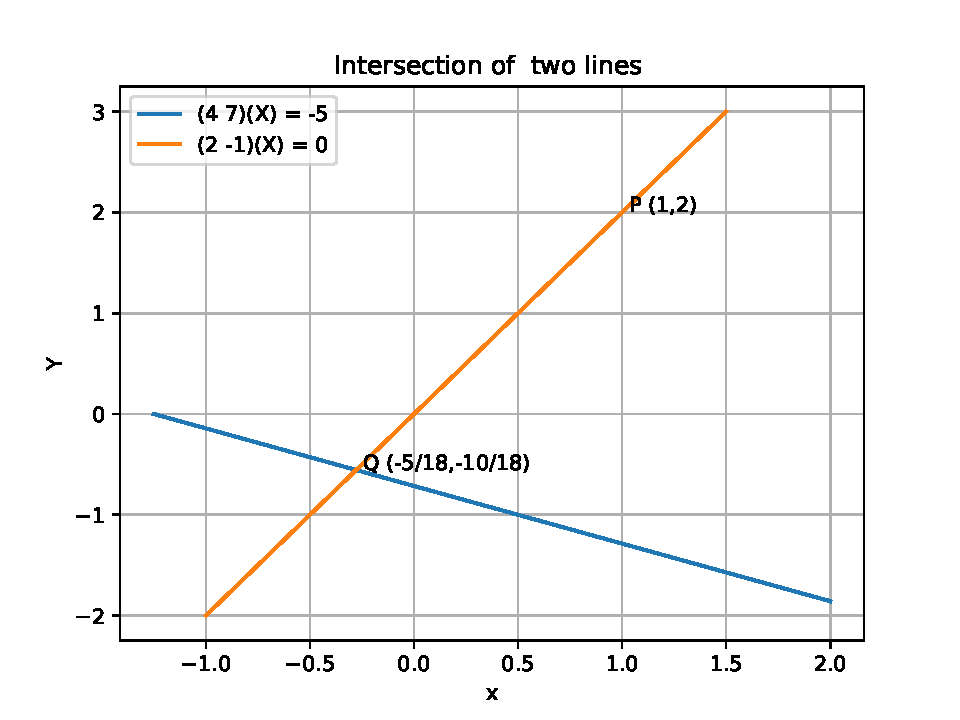
\includegraphics[width=.50\textwidth, height=.30\textheight]{./solutions/line_plane/52/Figure.pdf}	
	\caption{Intersection of two lines}
	\label{fig1:solutions/line_plane/52}	
\end{figure}


After solving this two equation we will get the  point of intersection, which is intersection of these two lines segments.
Thus, point of intersection is $\myvec {-5/18 \\ -10/18 \\ } $.
Now we have point of intersection
\begin{align}
 \vec{P} = 
\myvec{
-5/18\\
-10/18 \\	
}
\end{align}
and given point is
\begin{align}
\vec{Q}   = 
\myvec
{
1\\
2 \\	
} 
\end{align}
Now  the distance between two points is given as :
\begin{align}
\norm{
\vec{P} - \vec{Q}
} = 
\norm {
\myvec{
-5/18\\ 
-10/18 \\
}
-  \myvec {
1\\ 
2 \\
} }= d = 2.85 
\end{align}

